\documentclass[12pt,a4paper]{article}

% ==== Paket-Paket Ruwet Biar Berasa Hardcore ====
\usepackage[utf8]{inputenc}
\usepackage[T1]{fontenc}
\usepackage{lmodern}
\usepackage{geometry}
\usepackage{graphicx}
\usepackage{listings}
\usepackage{tabularx}
\usepackage{fancyhdr}
\usepackage{titlesec}
\usepackage{setspace}
\usepackage{xcolor}
\usepackage{enumitem}
\usepackage{float}
\usepackage{hyperref}
\usepackage{caption}
\usepackage{titling}
\usepackage{eso-pic}        % Tambahan untuk background
\usepackage{transparent}    % Transparansi gambar background
\usepackage{verbatim}
\usepackage{tikz}
\usetikzlibrary{positioning, arrows.meta}
\newcommand\BackgroundAllPages{%
  \AddToShipoutPicture{\BackgroundPic}
}

\lstset{
    basicstyle=\ttfamily\footnotesize,
    breaklines=true,
    backgroundcolor=\color{gray!10},
    frame=single,
    postbreak=\mbox{\textcolor{red}{$\hookrightarrow$}\space}
}


% ==== Geometry dan Margin ====
\renewcommand{\familydefault}{\sfdefault}
\newgeometry{top=2.5cm,bottom=3cm,left=3.5cm,right=2.5cm}

% ==== Variabel yang Bisa Diganti ====
\def\autor{Laboratorium}
\def\lab{Multimedia dan Internet of Things}
\def\departemen{Departemen Teknik Komputer}
\def\institut{Institut Teknologi Sepuluh Nopember}
\def\praktikum{Praktikum Jaringan Komputer}
\def\judul{Modul 2 – Routing dan Manajemen IPv6}
\def\nama{I Gusti Ngurah Opaldi Partha Dwipayana – 5024221057}
\def\tanggal{2025}

% ==== Background Setup ====
\newcommand\BackgroundPic{
  \put(0,0){
    \parbox[b][\paperheight]{\paperwidth}{
      \vfill
      \centering
      \transparent{0.1}
      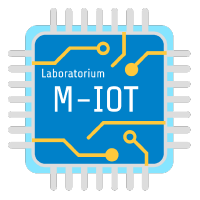
\includegraphics[width=0.5\paperwidth]{Cover/img/miot.png} % Ubah path jika perlu
      \vfill
    }
  }
}

\newcommand\BackgroundNone{%
  \ClearShipoutPicture
}

% ==== Heading Style ====
\titleformat{\section}{\normalfont\Large\bfseries}{\thesection}{1em}{}
\titleformat{\subsection}{\normalfont\large\bfseries}{\thesubsection}{1em}{}


\begin{document}

\BackgroundNone  % Hilangkan background untuk halaman judul

% ==== HALAMAN JUDUL ====
\begin{titlepage}
    \centering
    \begin{tabularx}{\textwidth}{l@{\hskip 0pt}lX}
        \raisebox{-0.5\height}{
\includegraphics[width=3cm]{Cover/img/logodepart.png}} 
        & \raisebox{-0.5\height}{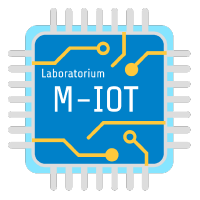
\includegraphics[width=3cm]{Cover/img/miot.png}} 
        & \raggedleft
        \begin{minipage}{0.5\textwidth}
            \raggedleft
            {\bfseries \small \autor} \\[-2pt]
            {\bfseries \small \lab} \\[-2pt]
            {\bfseries \small \departemen} \\[-2pt]
            {\bfseries \small \emph{\institut}}
        \end{minipage}
    \end{tabularx}
    
    \vspace{5cm}
    {\Huge \bfseries \praktikum \par}
    
    \vspace{2cm}
    {\LARGE \bfseries \judul \par}
    
    \vspace{2cm}
    {\Large \nama \par}
    
    \vfill
    {\Large \tanggal \par}
    
    \vfill
    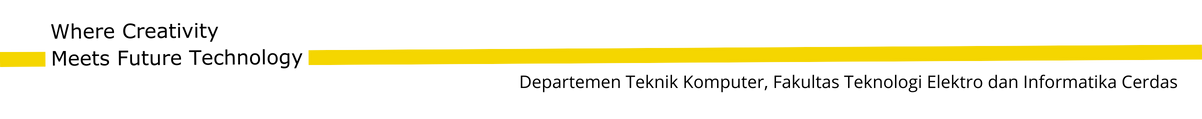
\includegraphics[width=\textwidth]{Cover/img/footer.png}
\end{titlepage}

\restoregeometry
\BackgroundAllPages
% Aktifkan background setelah halaman judul

% ==== KONTEN ====
\section{Pendahuluan}
\subsection{Latar Belakang}
Di era digital yang semakin maju dan serba terhubung seperti sekarang, hampir semua perangkat di dunia ingin “ngobrol” satu sama lain lewat internet. Mulai dari smartphone, komputer, bahkan kulkas dan jam tangan pintar pun terhubung secara online. Namun, di balik kemudahan ini, ada sebuah masalah yang sangat krusial: keterbatasan alamat IP. Sistem pengalamatan internet yang paling banyak digunakan selama ini, IPv4, hanya menyediakan sekitar 4,3 miliar alamat. Angka yang terdengar besar ini ternyata sudah tidak cukup lagi, mengingat jumlah perangkat yang ingin terhubung ke internet meningkat secara eksponensial setiap tahunnya.

Bayangkan jika semua perangkat yang ingin mengakses internet harus berbagi alamat yang sangat terbatas—hal ini seperti memiliki jalan raya yang cuma bisa dilewati oleh beberapa mobil saja, sementara kendaraan terus bertambah banyak setiap harinya. Kondisi ini membuat para ahli teknologi mulai mencari solusi yang bisa memberikan “jalan raya” yang jauh lebih lebar, agar semua perangkat bisa terhubung dengan lancar tanpa hambatan. Solusi itulah yang kemudian muncul dalam bentuk IPv6, protokol jaringan generasi terbaru yang dirancang khusus untuk menjawab masalah keterbatasan alamat di IPv4.

IPv6 bukan hanya soal menambah jumlah alamat yang tersedia, tapi juga membawa berbagai perbaikan penting, mulai dari pengaturan alamat yang lebih otomatis, keamanan yang lebih kuat, sampai efisiensi dalam pengiriman data. Dengan kemampuan menyediakan sekitar 340 undecillion alamat—angka yang hampir tidak terbayangkan—IPv6 membuka jalan bagi masa depan internet yang lebih luas, fleksibel, dan aman. Oleh karena itu, memahami teknologi IPv6 menjadi hal yang sangat penting untuk memastikan kita siap menghadapi tantangan jaringan di masa depan yang semakin kompleks dan masif.



\subsection{Dasar Teori}
Internet Protocol versi 6, atau IPv6, adalah sebuah lompatan besar dalam teknologi jaringan komputer. Jika IPv4 adalah “bahasa” yang digunakan internet selama beberapa dekade terakhir, maka IPv6 adalah versi terbaru yang membawa berbagai penyempurnaan dan inovasi. Perbedaan paling mencolok adalah pada panjang alamat IP—IPv6 menggunakan 128 bit, dibandingkan 32 bit pada IPv4. Hal ini membuat jumlah alamat yang tersedia meningkat drastis, dari miliaran menjadi triliunan kali lipat lebih banyak, yang bisa memenuhi kebutuhan dunia yang semakin digital.

Format alamat IPv6 memang terlihat kompleks pada awalnya, dengan delapan kelompok angka heksadesimal yang dipisahkan oleh tanda titik dua. Namun, format ini sebenarnya sangat terstruktur dan bahkan menyediakan aturan singkat untuk penulisan agar lebih mudah dibaca dan ditulis. IPv6 juga mendukung berbagai jenis alamat seperti unicast untuk satu perangkat, multicast untuk grup perangkat, dan anycast untuk mengirim ke perangkat terdekat dalam grup, yang membuat pengelolaan jaringan jadi lebih fleksibel dan efisien.

Salah satu keunggulan utama IPv6 adalah kemampuannya melakukan konfigurasi otomatis. Melalui mekanisme yang disebut Stateless Address Autoconfiguration (SLAAC), perangkat dapat langsung mengatur alamatnya sendiri tanpa perlu server khusus, membuat setup jaringan jadi jauh lebih simpel. Selain itu, IPv6 menyematkan fitur keamanan yang lebih kuat melalui IPsec sebagai standar, sehingga komunikasi data menjadi lebih terlindungi dari ancaman siber. Ditambah lagi, IPv6 mengoptimalkan cara data dikirim dan menangani mobilitas perangkat dengan lebih baik, yang sangat penting di era di mana perangkat bergerak bebas tanpa kehilangan koneksi.

Secara keseluruhan, IPv6 bukan sekadar protokol pengalamatan baru, tapi fondasi untuk internet masa depan yang lebih aman, lebih besar, dan lebih pintar. Dengan IPv6, kita bisa membayangkan dunia di mana segala perangkat, dari rumah pintar sampai kendaraan otonom, dapat terhubung tanpa batas, membuka berbagai kemungkinan baru yang selama ini hanya ada dalam imajinasi teknologi.


\section{Tugas Pendahuluan}
\begin{itemize}
    \item[1)] Jelaskan apa itu IPV6 dan apa bedanya dengan IPV4.
    \item[2)] Sebuah organisasi mendapatkan blok alamat IPv6 2001:db8::/32. a. Bagilah alamat tersebut menjadi empat subnet berbeda menggunakan prefix /64. b. Tuliskan hasil alokasi alamat IPv6 subnet untuk: - Subnet A - Subnet B - Subnet C - Subnet D
    
    \item [3)]Asumsikan terdapat sebuah router yang menghubungkan keempat subnet tersebut melalui empat antarmuka:
    \item[-] ether1 (Subnet A)
    \item[-] ether2 (Subnet B)
    \item[-] ether3 (Subnet C)
    \item[-]  ether4 (Subnet D) a. Tentukan alamat IPv6 yang akan digunakan pada masing-masing antarmuka router. b. Buatkan konfigurasi IP address IPv6 pada masing-masing antarmuka router.
    
    \item[4)] Buatlah daftar IP Table berupa daftar rute statis agar semua subnet dapat saling berkomunikasi.
    
    \item[5)] Jelaskan apa fungsi dari routing statis pada jaringan IPv6, dan kapan sebaiknya digunakan dibandingkan routing dinamis.
\end{itemize}

\subsection*{Jawaban :}
\begin{itemize}
    \item[1)] IPv6 (Internet Protocol version 6) adalah protokol jaringan terbaru yang dirancang untuk menggantikan IPv4 yang telah digunakan sejak awal pengembangan internet. IPv6 memungkinkan lebih banyak perangkat terhubung ke internet dengan menyediakan ruang alamat yang jauh lebih besar.

\subsection*{Perbedaan IPv6 dan IPv4}

\begin{center}
\begin{tabular}{|l|l|l|}
\hline
\textbf{Aspek} & \textbf{IPv4} & \textbf{IPv6} \\
\hline
Panjang Alamat & 32-bit & 128-bit \\
\hline
Format Alamat & Desimal (contoh: 192.168.1.1) & Hexadesimal (contoh: 2001:db8::1) \\
\hline
Jumlah Alamat & \textasciitilde 4,3 miliar & \textasciitilde 3.4 x 10\textsuperscript{38} \\
\hline
Konfigurasi Otomatis & Terbatas (DHCP) & SLAAC, DHCPv6 \\
\hline
Keamanan & Opsional & Wajib mendukung IPsec \\
\hline
Routing & Kurang efisien & Agregatif dan efisien \\
\hline
NAT & Digunakan luas & Tidak diperlukan \\
\hline
\end{tabular}
\end{center}

\item[2)] Organisasi mendapatkan blok alamat IPv6 yaitu 2001:db8::/32, yang merupakan blok alamat bersifat global (meskipun 2001:db8::/32 sendiri digunakan untuk dokumentasi dan simulasi). Blok ini memiliki prefix /32, yang berarti 32 bit pertama dari total 128 bit sudah tetap, dan 96 bit sisanya bisa digunakan untuk keperluan pengalamatan internal, termasuk subnetting.
\begin{itemize}
    \item a) Pembagian Menjadi Empat Subnet Berbeda Menggunakan Prefix /64
Untuk membagi blok 2001:db8::/32 menjadi empat subnet yang berbeda, kita perlu menambahkan 32 bit lagi agar setiap subnet memiliki panjang prefix /64, yang merupakan standar umum dalam jaringan IPv6. Dengan menggunakan 2 bit dari sisa ruang subnetting (karena 2² = 4), kita bisa membuat 4 kombinasi biner unik yang merepresentasikan 4 subnet berbeda. Bit-bit tambahan ini bisa kita tempatkan pada bagian keempat hextet (kelompok 16-bit), karena setelah 32 bit dari prefix awal, masih ada ruang 32 bit lagi untuk pengelompokan subnet sebelum mencapai /64.\\

\item b) Hasil Alokasi Alamat IPv6 untuk Setiap Subnet
Setelah proses pembagian dilakukan, maka diperoleh empat subnet dengan alokasi sebagai berikut:\\

Subnet A: \textbf{2001:db8:0:0::/64}
Subnet ini menggunakan semua bit tambahan sebagai nol, sehingga merupakan subnet pertama yang langsung mengikuti blok utama.\\

Subnet B: \textbf{2001:db8:0:1::/64}
Menggunakan satu bit tambahan, menghasilkan subnet kedua. Hextet keempat bernilai 0001.\\

Subnet C: \textbf{2001:db8:0:2::/64}
Kombinasi dua bit (10 dalam biner) menghasilkan nilai 2 dalam desimal pada hextet keempat.\\

Subnet D:\textbf{2001:db8:0:3::/64} 
Kombinasi biner 11 memberikan nilai hextet keempat menjadi 3, sehingga menjadi subnet keempat.

\end{itemize}

\item[3)] 
\subsection*{a) Penentuan Alamat IPv6 pada Antarmuka Router}
Setiap antarmuka router akan diberikan alamat IPv6 dalam subnet yang sesuai dengan subnet yang dihubungkannya. Biasanya, alamat yang digunakan adalah alamat pertama atau alamat host khusus di subnet tersebut untuk memudahkan identifikasi. Dengan asumsi menggunakan alamat host pertama setelah network prefix, maka konfigurasi alamat IPv6 untuk router adalah sebagai berikut:
\begin{center}
\begin{tabular}{|l|l|l|}
\hline
\textbf{Antarmuka} & \textbf{Subnet} & \textbf{Alamat IPv6 Router} \\
\hline
ether1 & Subnet A & \texttt{2001:db8:0:0::1/64} \\
\hline
ether2 & Subnet B & \texttt{2001:db8:0:1::1/64} \\
\hline
ether3 & Subnet C & \texttt{2001:db8:0:2::1/64} \\
\hline
ether4 & Subnet D & \texttt{2001:db8:0:3::1/64} \\
\hline
\end{tabular}
\end{center}

\subsection*{b) Konfigurasi IP Address IPv6 di Router}
Setiap antarmuka router akan diberikan alamat IPv6 dalam subnet yang sesuai dengan subnet yang dihubungkannya. Biasanya, alamat yang digunakan adalah alamat pertama atau alamat host khusus di subnet tersebut untuk memudahkan identifikasi. Dengan asumsi menggunakan alamat host pertama setelah network prefix, maka konfigurasi alamat IPv6 untuk router adalah sebagai berikut:
\subsubsection*{Contoh di Mikrotik:}
\begin{lstlisting}
/ipv6 address
add address=2001:db8:0:0::1/64 interface=ether1
add address=2001:db8:0:1::1/64 interface=ether2
add address=2001:db8:0:2::1/64 interface=ether3
add address=2001:db8:0:3::1/64 interface=ether4
\end{lstlisting}

\subsubsection*{Contoh di Cisco IOS:}
\begin{lstlisting}
interface GigabitEthernet0/0
 ipv6 address 2001:db8:0:0::1/64

interface GigabitEthernet0/1
 ipv6 address 2001:db8:0:1::1/64

interface GigabitEthernet0/2
 ipv6 address 2001:db8:0:2::1/64

interface GigabitEthernet0/3
 ipv6 address 2001:db8:0:3::1/64
\end{lstlisting}
\item[4)]Untuk memastikan semua subnet dapat saling berkomunikasi, diperlukan konfigurasi daftar rute statis (static routing) pada router. Rute statis adalah aturan routing yang secara manual mengarahkan paket ke subnet tujuan melalui antarmuka yang sesuai. Berikut adalah contoh konfigurasi rute statis pada router:

\begin{itemize}
    \item Rute langsung untuk Subnet A (\texttt{2001:db8:0:0::/64}) melalui \texttt{ether1}
    \item Rute statis untuk Subnet B (\texttt{2001:db8:0:1::/64}) melalui \texttt{ether2}
    \item Rute statis untuk Subnet C (\texttt{2001:db8:0:2::/64}) melalui \texttt{ether3}
    \item Rute statis untuk Subnet D (\texttt{2001:db8:0:3::/64}) melalui \texttt{ether4}
\end{itemize}

Konfigurasi ini memastikan paket data dari satu subnet dapat diteruskan dengan benar ke subnet lain melalui router.

\subsection*{Contoh konfigurasi routing statis Mikrotik:}
\begin{lstlisting}
/ipv6 route
add dst-address=2001:db8:0:1::/64 gateway=ether2
add dst-address=2001:db8:0:2::/64 gateway=ether3
add dst-address=2001:db8:0:3::/64 gateway=ether4
\end{lstlisting}




\item[5)] Routing statis pada jaringan IPv6 adalah metode pengaturan jalur routing yang dilakukan secara manual oleh administrator jaringan. Fungsi routing statis antara lain:

\begin{itemize}
    \item Memberikan kontrol penuh atas jalur routing sehingga sangat cocok untuk jaringan kecil dan topologi yang stabil.
    \item Meningkatkan keamanan dan prediktabilitas karena jalur routing tidak berubah kecuali diubah secara manual.
    \item Menghemat sumber daya perangkat router karena tidak memerlukan protokol routing dinamis yang kompleks.
\end{itemize}

Routing statis sebaiknya digunakan ketika:

\begin{itemize}
    \item Jaringan berskala kecil dan jarang mengalami perubahan topologi.
    \item Administrator menginginkan jalur routing yang tetap dan tidak berubah demi alasan keamanan atau kestabilan.
    \item Sumber daya perangkat terbatas sehingga tidak mendukung routing dinamis.
\end{itemize}

Sebaliknya, routing dinamis lebih efektif digunakan pada jaringan besar dengan topologi yang kompleks dan sering berubah, karena protokol routing dinamis dapat memperbarui jalur secara otomatis.










\end{itemize}
\end{document}
